
\chapter{Интегрирование на промежутке}

Понятие определённого интеграла восходит ещё к Архимеду. Мы рассмотрим неформальное введение, где объясним суть проблемы.

\section{Неформальное введение}

Пусть дана функция $f: \mathbb{R} \to \mathbb{R}^1$, которая непрерывна на отрезке $[a,b]$. Будем писать $y  = f(x)$ и будем считать, что функция на этом отрезке принимает только положительные значения. Рассмотрим фигуру $ABCD$ (см. рис.\ref{int_a_b}), ограниченную кривой $y=f(x)$, двумя ординатами $x = a$, $x =b$ и отрезком оси $Ox.$ Подобные фигуры называются \textit{криволинейными трапециями}.

Рассмотрим теперь задачу о нахождении площади плоской криволинейной трапеции $ABCD$ (см. рис.\ref{int_a_b})

\begin{figure}[h!]
    \centering
    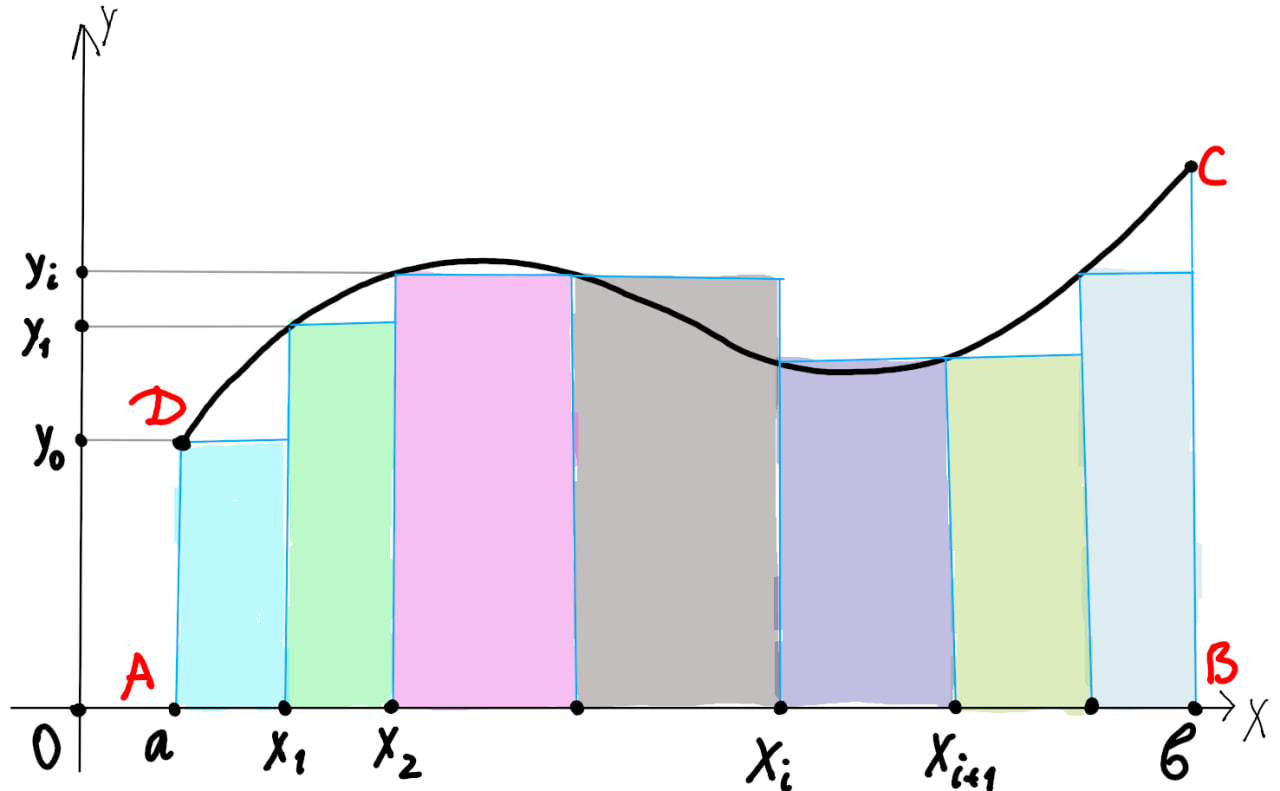
\includegraphics[scale=0.5]{int_a_b1.jpg}
    \caption{Площадь фигуры $ABCD$ примерно равна сумме площадей разноцветных прямоугольников, и чем их больше, тем точнее будет ответ.}
    \label{int_a_b}
\end{figure}

Разделим основание $AB$ нашей фигуры произвольным образом на части и проведём ординаты, соответствующие точкам деления; тогда криволинейная трапеция разобьётся на ряд полосок. 

Заменим теперь приближённо каждую полоску некоторым прямоугольником, основание которого то же, что и у полоски, а высота совпадает с одной из ординат полоски. Таким образом, криволинейная фигура заменится некоторой ступенчатой фигурой, составленной из отдельных прямоугольников. 

Обозначим абсциссы точек деления через
\[
 x_0 : = a < x_1 < x_2 < \cdots < x_i < x_{i+1} < \cdots < x_n =:b.
\]

Будем нумеровать прямоугольники числами $0,1,2,\ldots, n-1$ и пусть $S_i$ -- площадь $i$-го прямоугольника. Ясно, что $S_i = y_i \Delta x_i$, где $\Delta x_i: = x_{i+1} - x_i.$

Тогда приближённое значение площади криволинейной трапеции $S_{ABCD}$ равно
\[
 S_{ABCD} \approx \sum_{k = 0}^{n-1} y_k \Delta x_k.
\]

Тогда можно предположить, что при убывании всех $\Delta x_i$ к нулю мы будем получать более точное значение, \textit{т.е.} другими словами мы хотим сказать, что точное значение площади это следующий предел
\[
 S_{ABCD} = \lim_{\substack{\Delta x_1 \to 0 \\ \vdots \\ \Delta x_{n-1} \to 0}} \sum_{k = 0}^{n-1} y_k \Delta x_k.
\]

Для обозначения предела такой суммы вида и был Лейбницем введён символ интеграла, \textit{т.е.}
\[
 \int_a^b f(x) \mathrm{d}x : = \lim_{\substack{\Delta x_1 \to 0 \\ \vdots \\ \Delta x_{n-1} \to 0}} \sum_{k = 0}^{n-1} y_k \Delta x_k.
\]


\section{Интеграл ступенчатой функции.}

Предыдущее ``определение'' интеграла имеет очень много недостатков. Например, мы пользовались интуитивным пониманием площади криволинейной трапеции. 

Здесь мы дадим строгое определение интеграла.

\subsection{Разбиение промежутка} Напомним, что под промежутком мы понимаем подмножество прямой $\mathbb{R}$ одного из видов; $[a,b]$, $[(a,b]$, $[a,b)$, $(a,b)$, при этом мы считаем, что $|a|,|b| < \infty.$ Промежуток мы будем обозначать буквами $I$ или $J$, а под \textit{длиной промежутка} будем понимать выражение, $b-a$ и если $I$ один из рассмотренных промежутков, то будем писать $|I|: = b-a.$

\begin{mydanger}{\bf !}
    Нам также будет полезно рассматривать пустой промежуток $I$ или, если он содержит всего одну точку, то в таком случае полагаем $|I|:=0$.
\end{mydanger}

\begin{definition}
    Пусть $I$ -- промежуток, под \textit{разбиением} промежутка $I$ понимается \textbf{конечное} множество $\lambda(I)$ промежутков содержащихся в $I$, при этом любой $x \in I$ принадлежит одному и только одному промежутку из $\lambda.$
\end{definition}

\begin{example}
  Пусть $I = [1,8]$, тогда следующее множество
  \[
   \lambda(I) : = \{ \varnothing, \{1\}, (1,3), [3,5), \{5\}, (5,8]  \}
  \]
есть разбиение промежутка $I = [1,8]$, потому что любой $x \in I$ лежит в одном и только в одном из перечисленных подмножеств множества $\lambda(I)$. А если же мы положим, что
\[
 \lambda'(I): = \{ \varnothing, \{1\}, [1,3), (2,7), [3,5), \{5\}, (5,8] \}
\]
то мы уже получаем не разбиение, поскольку, например, точка $2.5 \in [1,3)$ и $2.5 \in (2,7)$.

Множество $\lambda''(I) := \{[1,4), (4,8]\}$ тоже не является разбиением промежутка $I = [1,8]$ так как $4$ не принадлежит ни одному из подмножеств множества $\lambda''(I)$. Наконец, множество $\lambda'''(I) := \{(0,5], (5,8]\}$ также не является разбиением промежутка $I = [1,8]$, потому что $(0,5]$ не содержится в $I.$
\end{example}

\begin{mydanger}{\bf !}
    Заметим, что пустое множество может не входить в разбиение промежутка. 
\end{mydanger}


\begin{theorem}[Конечная аддитивность длины]\label{additive_of_lenght}
    Пусть $I\subsetneq \mathbb{R}$ -- промежуток, а $\lambda(I)$ -- его разбиение, тогда
    \[
     |I| = \sum_{A \in \lambda(I)}|A|.
    \]
\end{theorem}
\begin{proof}
Доказывать будем по индукции, а именно по мощности разбиения. То есть для всех разбиений, в которых ровно $n$ элементов верна формула $|I| = \sum_{A \in \lambda(I)}|A|$.

(1) Если $n =0$ то значит, что $I = \varnothing$, так как любое его разбиение не должно иметь непустых элементов, но тогда формула очевидна.

(2) Если $n=1$, то это значит, что любое его разбиение имеет ровно один непустой элемент, а это значит, что $I = \{a\}$ -- одноточечное множество, но и в таком случае формула тоже очевидна.

(3) Пусть формула верна для любых разбиений, в которых ровно $n\ge 1$ элементов. И допустим теперь, что у промежутка $I$ имеются разбиения, у которых $n+1$ элементов. Именно для таких разбиений мы будем доказывать формулу. Случаи, когда $I = \varnothing$ или же когда $I = \{a\}$ очень просты для рассмотрения, так как тогда все разбиения либо содержат пустое множество, либо пустое и одноточечное.

Итак, пусть $I$ -- это одно из четырёх множеств $(a,b), (a,b], [a,b), [a,b]$.

Допустим, что $b \in I$ тогда $I$ -- это либо $(a,b]$, либо $[a,b]$. Рассмотрим произвольное разбиение $\lambda(I)$, в котором ровно $n+1$ элементов, тогда должен найтись ровно один элемент, скажем, $B$, который содержит $b$.

С другой же стороны, $B \subseteq I$, а тогда $B$ имеет либо вид $(c,b]$, либо $[c,b]$ или же $\{b\}$, где $a \le c \le b$. Для удобства можно считать, что в последнем случае $c =b$.

Рассмотрим теперь множество $I \setminus B$, которое имеет вид либо $[a,c]$, либо $(a,c)$, либо $(a,c]$, или $[a,c)$, когда $c >a$, или же $I \setminus B$ -- это точка или пустое множество. Другими словами, $I\setminus B$ -- это промежуток. 

Далее, так как $I = B \cup I \setminus B$ и $B \cap I \setminus B = \varnothing$, то множество $\lambda(I) \setminus B$ является разбиением промежутка $I\setminus B$. 

Таким образом, разбиение $\lambda(I)\setminus B$ содержит уже $n$ элементов. Но согласно предположению, для промежутка $I \setminus B$ верна формула
\[
 |I \setminus B| = \sum_{K \in \lambda(I) \setminus B} |K|
\]

Воспользовавшись теперь равенством,
\[
 |I| =|B| + |I \setminus B|
\]
мы получим

\[
 |I| = |B| + |I \setminus B| = |B| + \sum_{K \in \lambda(I) \setminus B} |K| = \sum_{A \in \lambda(I)} |A|.
\]

(4) Осталось рассмотреть случай, когда $b \notin I$, но тогда $I$ это либо $(a,b)$ либо $[a,b)$ и существует один из элементов множества $\lambda(I)$ который имеет вид либо $(c,b)$ или же $[c,b)$. Это означает, что вид множества $I \setminus B$ может принять одно из четырёх значений $[a,c]$, $(a,c)$, $(a,c]$, $[a,c)$ когда $c >a$ или же это точка или пустое множество. Остальная часть рассуждения продолжается как выше. 
\end{proof}


Эту теорему легко обобщить следующим образом.
\begin{lemma}\label{additive_of_a-lenght}
 Пусть $\alpha: I \to \mathbb{R}$ -- непрерывная функция, а $I$ -- ограниченный промежуток одного из вида $(a,b), [a,b], (a,b], [a,b)$, тогда положим
 \[
  \alpha(I): = \alpha(b) - \alpha(a).
 \]
Тогда для любого разбиения $\lambda(I)$ имеем
\[
 \alpha(I) = \sum_{A \in \lambda(I)}\alpha(A).
\]
\end{lemma}
\begin{proof}[Набросок доказательства]
    Рассуждения такие же как и в предыдущей лемме, но нужно использовать очевидное наблюдение, если $B  = [c,b] \subseteq I = [a,b]$, то $I\setminus B = [a,c)$ и тогда
    \begin{eqnarray*}
        \alpha(B) + \alpha(I \setminus B) &=& \alpha(b) - \alpha (c) + \alpha (c) + \alpha(a) \\
        &=& \alpha(b) -\alpha(a) \\
        &=& \alpha(I).
    \end{eqnarray*}
\end{proof}
 


\subsection{Ступенчатые функции}

Сейчас мы опишем класс функций, которые ``очень просты'' для интегрирования\footnote{Отметим, что эти функции также ещё называются \textit{кусочно-постоянными}, в англоязычной литературе они так и называются, \textit{piecewise constant functions.}}, а потом с помощью их мы уже определим интеграл в общем виде.  

\begin{definition}
  Пусть $A \subseteq \mathbb{R}$, и пусть дана функция $f: A \to \mathbb{R}$. Говорят, что $f$ \textit{постоянная функция}, если существует такое $\alpha \in \mathbb{R}$, что $f(x) = \alpha$ для всех $x \in A$. Если $B \subseteq A$, то говорят, что $f$ \textit{постоянная на $B$}, если существует такое $\beta \in \mathbb{R}$, что $f(y) = \beta$ для всех $y \in B.$
\end{definition}


\begin{mydanger}{\bf !}
 Из этого определения следует, что если функция $f$ постоянна на \textbf{непустом} множестве $A$, то она не может принимать два или более разных значения. Однако из определения пустого множества следует, что постоянная функция на пустом множестве может принимать \textbf{любое значение!}
\end{mydanger}

\begin{definition}
    Пусть дан промежуток $I \subsetneq \mathbb{R}$, и пусть дана функция $f: I \to \mathbb{R}$, и пусть $\lambda(I)$ -- какое-то разбиение промежутка $I$. Говорят, что \textit{функция $f$ есть ступенчатая функция на $I$ относительно $\lambda(I)$}, если для каждого $J \in \lambda(I)$, $f$ является постоянной на $J$. 
\end{definition}

\begin{example}\label{int_[1,6]=10}
    Пусть $I = [1,6]$ и определим функцию $f: [1,6]: \to \mathbb{R}$ следующим образом
    \[
     f(x) = \begin{cases}
         \,7, & 1 \le x < 3 \\
         \,4, & x = 3 \\
         \,5, & 3 < x <6 \\
         \,2, & x = 6.
     \end{cases}
    \]
Тогда, если мы рассмотрим разбиение
\[
 \lambda(I) := \Bigl\{[1,3), \{3\}, (3,6), \{6\} \Bigr\}
\]
промежутка $I$, то получаем, что $f$ -- ступенчатая функция относительно этого разбиения. Рассмотрим теперь другое разбиение этого же промежутка
\[
 \lambda'(I) : = \Bigl\{\varnothing, [1,2), \{2\}, (2,3), \{3\}, (3,5), [5,6),\{6\} \Bigr\}.
\]
Тогда несложно видеть, что $f$ будет тоже ступенчатой относительно этого разбиения. 
\end{example}

Этот пример показывает, что понятие ступенчатой функции можно определить без привлечения разбиения промежутка.

\begin{definition}\label{fiber}
Пусть $I$ -- промежуток, и пусть $\lambda(I)$, $\lambda'(I)$ -- два его разбиения. Говорят, что разбиение $\lambda'(I)$ \textit{тоньше}, чем $\lambda(I)$, если для каждого $J' \in \lambda'(I)$ найдётся такой $J \in \lambda(I)$, что $J' \subseteq J$.
\end{definition}

\begin{example}
 Вернёмся к предыдущему примеру с промежутком $I = [1,6]$ и разбиениями   
 \begin{eqnarray*}
     \lambda(I) &:=& \Bigl\{[1,3), \{3\}, (3,6), \{6\} \Bigr\},\\
     \lambda'(I) &: =& \Bigl\{\varnothing, [1,2), \{2\}, (2,3), \{3\}, (3,5), [5,6),\{6\} \Bigr\}.
 \end{eqnarray*}

Тогда видно, что $\lambda'(I)$ тоньше, чем $\lambda(I)$.
\end{example}


\begin{definition}
    Пусть дан промежуток $I \subsetneq \mathbb{R}$ и пусть дана функция $f: I \to \mathbb{R}$. Говорят, что функция $f$ \textit{ступенчатая на $I$}, если существует такое разбиение $\lambda(I)$, что $f$ -- постоянная на $I$ относительно $\lambda(I).$
\end{definition}


\begin{lemma}\label{fiber_for_functions}
  Пусть $I \subsetneq \mathbb{R}$ -- промежуток и пусть $f:I \to \mathbb{R}$ -- ступенчатая функция относительно разбиения $\lambda(I)$, тогда если имеем разбиение $\lambda'(I)$, которое тоньше, чем $\lambda(I)$, то $f$ -- ступенчатая относительно $\lambda'(I).$ 
\end{lemma}

\begin{proof}
    Действительно, пусть $A' \in \lambda'(I)$ -- произвольный элемент разбиения, тогда найдётся такой $A \in \lambda(I)$, что $A' \subseteq A$. Тогда если $f(x) = \alpha$ для всех $x \in A$, то и $f(x') = \alpha$ для всех $A'.$
\end{proof}

\begin{mydanger}{\bf !}
    Таким образом, мы будем рассматривать просто ступенчатые функции на промежутке, не определяя какое-то конкретное разбиение.
\end{mydanger}


В связи с этим уместно ввести следующее важное для дальнейшего определение.

\begin{definition}
    \textit{Характеристической функцией} некоторого множества $A \subseteq X$ называется функция $\chi_A: X\to \{0,1\}$ определённая следующим образом
    \[
     \chi_A(x): = \begin{cases}
         1 & x \in A, \\
         0 & x \notin A.
     \end{cases}
    \]
\end{definition}

\begin{remark}
 Таким образом, если $f: I \to \mathbb{R}$ -- ступенчатая функция на промежутке $I$ и пусть $\lambda(I)$ -- соответствующее разбиение промежутка $I$, тогда мы можем записать
 \[
  f =\sum_{A \in \lambda(I)} f(A) \cdot \chi_A.
 \]
\end{remark}

\begin{mydanger}{\bf !}
    Из определения следует, что $\chi_{\varnothing} = 0$, так как не существует такого $x$ чтобы $x \in \varnothing.$
\end{mydanger}


\begin{lemma}\label{chi_A+chi_B}
    Пусть $A$, $B$ два подмножества множества $X$, тогда 
    \begin{eqnarray*}
        \chi_{A \cup B} = \chi_A + \chi_B - \chi_{A\cap B},\\
        \chi_{A \cap B} = \chi_A \cdot \chi_B,\\
        \chi_{A^c} = 1 - \chi_A.
    \end{eqnarray*}
\end{lemma}

\begin{proof} (1) Пусть $x \in A\cap B$, то $x\in A$, $\chi_B$, \textit{т.е.} $\chi_A(x) = \chi_B(x) = 1$. Если $x \notin A \cup B$, то $x\notin A$, $x\notin B$ и тогда $\chi_A(x) = \chi_B(x) = 0$. В любом из этих случаев имеем $\chi_{A \cap B}(x) = \chi_A(x) \cdot \chi_B(x).$ 

(2) Пусть $x \in A^c$, тогда $x\notin A$, тогда \textit{т.е.} $\chi_{A^c}=1$, $\chi_A(x) = 0$. Если $x \notin A^c$, то $x \in A$, \textit{т.е.} $\chi_{A^c}=0$, $\chi_A(x) = 1$, что и доказывает формулу $\chi_{A^c} = 1 - \chi_A.$

(3) Наконец, так как $(A \cup B)^c = A^c \cap A^c$, то используя результаты выше, получаем
\begin{eqnarray*}
    \chi_{A \cup B} &=& 1 - \chi_{(A\cup B)^c} \\
    &=& 1 - \chi_{A^c \cap B^c} \\
    &=& 1- \chi_{A^c} \cdot \chi_{B^c} \\
    &=& 1 - (1- \chi_A)(1-\chi_B) \\
    &=& 1 - (1-\chi_B - \chi_A + \chi_{A}\cdot \chi_B) \\
    &=& 1 - 1 + \chi_A + \chi_B - \chi_{A \cap B} \\
    &=&\chi_A + \chi_B - \chi_{A \cap B}.
\end{eqnarray*}
\end{proof}


\begin{example}

Вернёмся к примеру \ref{int_[1,6]=10}, имеем $I = [1,6]$ и функцию $f: [1,6]: \to \mathbb{R}$;
    \[
     f(x) = \begin{cases}
         \,7, & 1 \le x < 3 \\
         \,4, & x = 3 \\
         \,5, & 3 < x <6 \\
         \,2, & x = 6.
     \end{cases}
    \]
Как мы уже видели, $f$ -- ступенчатая относительно разбиений
\begin{align*}
    &  \lambda(I) := \Bigl\{[1,3), \{3\}, (3,6), \{6\} \Bigr\},\\
    &  \lambda'(I) : = \Bigl\{\varnothing, [1,2), \{2\}, (2,3), \{3\}, (3,5), [5,6),\{6\} \Bigr\}.
\end{align*}

Тогда получаем, что
\[
 f = 7 \cdot \chi_{[1,3)} + 4 \cdot \chi_{\{3\}} + 5 \cdot \chi_{(3,6)} + 2 \cdot \chi_{\{6\}},  
\]
а также
\[
f = \alpha \cdot \chi_{\varnothing} + 7 \cdot \chi_{[1,2)} + 7 \cdot \chi_{\{2\}} + 7 \cdot \chi_{(2,3)} + 4 \cdot \chi_{\{3\}} + 5 \cdot \chi_{(3,5)} + 5 \cdot \chi_{[5,6)} + 2 \cdot \chi_{\{6\}},
\]
где $\alpha \in \mathbb{R}$ -- произвольное число, но так как $\chi_\varnothing = 0$, то всё корректно.
\end{example}

\begin{proposition}\label{beautefull}
    Пусть имеем две ступенчатые функции $f,g:I \to \mathbb{R}$ и пусть $\lambda_f(I) = \cup_{p=1}^n A_p$, $\lambda_g(I) = \cup_{q=1}^m B_q$ -- разбиения промежутка $I$ такие, что $f$, $g$ -- ступенчаты относительно $\lambda_f(I)$ и $\lambda_g(I)$ соответственно. Тогда $\lambda(I): = \cup_{p=1}^n \cup_{q=1}^m A_p \cap B_q$ -- разбиение промежутка $I$, и более того каждая из функций $f,g$ ступенчата относительно него и
    \begin{align*}
        & f =  \sum_{p=1}^n\sum_{q=1}^m f(A_p) \cdot \chi_{A_p}\cdot \chi_{B_q}\\
        & g=  \sum_{p=1}^n\sum_{q=1}^m g(B_q) \cdot \chi_{A_p} \cdot \chi_{B_q}.
    \end{align*}
\end{proposition}

\begin{proof} Покажем, что это разбиение. Так как $I = \cup_{p=1}^n A_p = \cup_{q= 1}B_q$, то
\[
 \cup_{p=1}^n \cup_{q=1}^m A_p \cap B_q  = \left( \cup_{p=1}^n A \right) \cap \left( \cup_{q=1}^m B_q \right) = I \cap I = I,
\]
в силу того, что $A_p \cap A_{p'} = \varnothing$ и $B_q \cap B_{q'} = \varnothing$, то $(A_p \cap B_q) \cap (A_{p'}\cap B_{q'}) = \varnothing$, $1\le p \le n$, $1\le q \le m$. Поэтому $\lambda(I)$ -- разбиение промежутка $I$.


Далее, так как $\lambda_f(I)$, $\lambda_g(I)$ разбиения, то для любых $1\le p \le n$, $1\le q \le m$, имеем
\[
 A_p = \cup_{q=1}^m (A_p \cap B_q), \qquad B_q = \cup_{p=1}^n (A_p \cap B_q).
\]

Наконец, так как $\chi_\varnothing = \varnothing$, и пользуясь леммой \ref{chi_A+chi_B}, получаем
\begin{eqnarray*}
    f &=& \sum_{p=1}^n f(A_p) \cdot \chi_{A_p} \\
    &=& \sum_{p=1}^n\sum_{q=1}^m f(A_p) \cdot \chi_{ \cup_{q=1}^m (A_p \cap B_q)} \\
    &=& \sum_{q=1}^m f(A_p) \cdot \left(\chi_{A_p \cap B_1} + \cdots + \chi_{A_p \cap B_m} \right) \\
    &=& \sum_{p=1}^n\sum_{q=1}^m f(A_p) \cdot \chi_{A_p \cap B_q}.
\end{eqnarray*}

Аналогично доказывается формула для функции $g.$
    
\end{proof}


\begin{corollary}\label{cor_for_sum}
 Пусть $I \subsetneq \mathbb{R}$ -- промежуток и пусть $f,g:I \to \mathbb{R}$ -- ступенчатые функции на нём. Тогда функции
    \[
     f\pm g, \quad \max\{f,g\}, \quad f\cdot g
    \]
    тоже ступенчатые на $I$. Если $g(x) \ne 0$ при $x \in I$, то $\frac{f}{g}$ тоже ступенчатая функция на $I.$    
\end{corollary}
    

\begin{proof}

Пусть $\lambda_f(I)  =  \cup_{p=1}^n A_p$, $\lambda_g(I) =  \cup_{q=1}^m B_q$ -- разбиения промежутка $I$ относительно которых $f$, $g$ -- ступенчаты, соответственно. Согласно предложению \ref{beautefull},
  \begin{align*}
        & f =  \sum_{p=1}^n\sum_{q=1}^m f(A_p) \cdot \chi_{A_p}\cdot \chi_{B_q}\\
        & g=  \sum_{p=1}^n\sum_{q=1}^m g(B_q) \cdot \chi_{A_p} \cdot \chi_{B_q}.
    \end{align*}

Тогда, получаем
\begin{eqnarray*}
    f \pm g &=& \sum_{p=1}^n\sum_{q=1}^m (f(A_p) \pm g(B)q) \cdot \chi_{A_p}\cdot \chi_{B_q} \\
     \max\{f ,g\} &=& \sum_{p=1}^n\sum_{q=1}^m \max\{f(A_p), g(B)q)\} \cdot \chi_{A_p}\cdot \chi_{B_q},\\
      f \cdot g &=& \sum_{p=1}^n\sum_{q=1}^m (f(A_p) \cdot g(B)q) \cdot \chi_{A_p}\cdot \chi_{B_q},\\
     \frac{f}{ g} &=& \sum_{p=1}^n\sum_{q=1}^m \left(\frac{f(A_p)}{ g(B_q)}\right) \cdot \chi_{A_p}\cdot \chi_{B_q},\qquad g \ne 0,
\end{eqnarray*}
что и требовалось доказать.
\end{proof}

\subsection{Интеграл от ступенчатой функции на промежутке}

Итак, у нас всё готово, чтобы ввести следующее важное определение.

\begin{definition}\label{int_of_p.c_on_I}
    Пусть $I \subsetneq \mathbb{R}$ -- промежуток, $\lambda(I)$ -- разбиение промежутка $I$ и пусть $f:I \to \mathbb{R}$ -- ступенчатая функция относительно этого разбиения, \textit{т.е.} $f = \sum_{A \in \lambda(I)}f(A) \cdot \chi_A$. Определим \textit{интеграл на промежутке $I$} ступенчатой функции $f:I \to \mathbb{R}$ относительно разбиения $\lambda(I)$ следующим образом
    \[
     \int_{\lambda(I)}f: =  \sum_{A \in \lambda(I)} f(A)\cdot |A|
    \]
\end{definition}

\begin{mydanger}{\bf !}
     Во-первых, что стоит слева от равно нужно понимать как символ и не более того! Во-вторых, это определение может показаться некорректным если $\lambda(I)$ содержит пустое множество, но так как $|\varnothing| = 0$, то мы на самом деле получаем корректное определение.     
\end{mydanger}

\begin{remark}\label{int_via_chi}
    Если $f = \chi_I$, и взяв разбиение $\lambda(I) = \{I\}$ то мы получаем следующее
    \[
     \int_{\lambda(I)}\chi_I = |I|.
    \]
И тогда мы можем записать, что если $f = \sum_{A \in \lambda(I)}f(A) \cdot \chi_A$, то
\[
\boxed{
 \int_{\lambda(I)}f = \sum_{A \in \lambda(I)} f(A) \cdot \int_{\lambda(I)}\chi_A
 }
\]
\end{remark}


\begin{example}\label{int_[1,4]=10}
    Пусть $f: [1,4] \to \mathbb{R}$ определена следующим образом
    \[
     f(x)  = \begin{cases}
          \, 2 & 1 \le x <3 \\
          \, 4 & x = 3 \\
          \, 6 & 3< x \le 4
     \end{cases}
    \]
    и пусть $\lambda(I) = \{ [1,3), \{3\}, (3,4] \}$, тогда
 \begin{eqnarray*}
  \int_{\lambda(I)} f  &=& \alpha_{[1,3)}\cdot | [1,3) | + \alpha_{\{3\}}\cdot |\{3\}| + \alpha_{(3,4]} \cdot | (3,4] | \\
  &=& 2 \cdot 2 + 4 \cdot 0 + 6 \cdot 1 \\
  &=& 10.
 \end{eqnarray*}

 С другой стороны, рассмотрим такое разбиение $\lambda'(I) = \{ \varnothing, [1,2), [2,3), \{3\}, (3,4] \}$, нетрудно видеть, что оно тоньше разбиения $\lambda(I)$. Находим
 \begin{eqnarray*}
     \int_{\lambda'(I)}f &=&\alpha_\varnothing \cdot |\varnothing| + \alpha_{[1,2)} \cdot | [1,2) | + \alpha_{[2,3)} \cdot |[2,3)| + \alpha_{\{3\}}\cdot |\{3\}| + \alpha_{(3,4]} \cdot | (3,4] | \\
     &=& \alpha_\varnothing \cdot 0 + 2 \cdot 1 + 2 \cdot 1 + 4 \cdot 0 + 6 \cdot 1 \\
     &=& 10.
 \end{eqnarray*}
 
\end{example}

Итак, мы увидели, что, взяв разбиение тоньше, значение интеграла не изменилось, очевидно, что это верно и в общем случае.

\begin{lemma}
  Пусть $I \subsetneq \mathbb{R}$ -- промежуток и пусть $f:I \to \mathbb{R}$ -- ступенчатая функция относительно разбиения $\lambda(I)$, тогда если имеем разбиение $\lambda'(I)$, которое тоньше, чем $\lambda(I)$, то
  \[
   \int_{\lambda(I)}f = \int_{\lambda'(I)}f.
  \]
\end{lemma}

\begin{proof}
    Пусть $\lambda(I) = \{ A_1,\ldots, A_n \}$ и пусть 
    \[
     \lambda'(I) : = \Bigl\{A_{11}', \ldots, A'_{1\ell_1},\ldots, A'_{n1},\ldots, A'_{n\ell_n} \Bigr\},
    \]
    где $A_i$ содержит только $A'_{i1},\ldots, A'_{i\ell_i}$, $1\le i \le n$. Из определения \ref{fiber} тогда следует, что $A_i = A'_{i1} \cup \cdots \cup A'_{i\ell_i}$ и $|A_i| = |A'_{i1}| + \cdots + |A'_{i\ell_i}|$.
    
    Наконец, используя лемму \ref{fiber_for_functions}, получаем, что
    \[
     f(A'_{i1}) = \cdots = f(A'_{i\ell_i}) = f(A_i), \qquad 1 \le i \le \ell.
    \]

    Таким образом, имеем
    \begin{eqnarray*}
        \int_{\lambda'(I)}f &=& \Bigl(f(A_{11}') \cdot \left| A'_{11} \right| + \cdots + f(A_{1\ell_1})\cdot \left|A'_{i\ell_1}\right|\Bigr) + \cdots + \Bigl(f(A_{11}') \left|A_{11}'\right| + \cdots + f(A_{1\ell_1})\cdot \left|A'_{i\ell_1}\right| \Bigr) \\
        &=& f(A_1) \cdot \left( \left| A'_{11}  \right| + \cdots + \left| A'_{1\ell_1} \right| \right) + \cdots + f(A_n) \cdot \left( \left| A'_{n1}  \right| + \cdots + \left| A'_{n\ell_n} \right| \right) \\
        &=& f(A_1) |A_1| + \cdots + f(A_n)\cdot |A_n| \\
        &=& \int_{\lambda(I)}f.
    \end{eqnarray*}
\end{proof}


Таким образом, мы можем ввести следующее определение, которое будем использовать в дальнейшем.

\begin{definition}\label{int_of_p.c}
    Пусть $I \subsetneq \mathbb{R}$ -- промежуток, $f:I \to \mathbb{R}$ -- ступенчатая функция на нём. Определим \textit{интеграл на промежутке $I$} ступенчатой функции $f:I \to \mathbb{R}$ следующим образом
    \[
     \int_If: =  \int_{\lambda(I)}f,
    \]
    где $\lambda(I)$ такое разбиение промежутка $I$, что $f$ является ступенчатой относительно $\lambda(I).$
\end{definition}


\begin{example}
Вернёмся к примеру \ref{int_[1,4]=10}. Пусть $f: [1,4] \to \mathbb{R}$ определена следующим образом
    \[
     f(x)  = \begin{cases}
          \, 2 & 1 \le x <3 \\
          \, 4 & x = 3 \\
          \, 6 & 3< x \le 4
     \end{cases}
    \]
    и пусть $\lambda(I) = \{ [1,3), \{3\}, (3,4] \}$, тогда
 \begin{eqnarray*}
  \int_{\lambda(I)} f  &=& \alpha_{[1,3)}\cdot | [1,3) | + \alpha_{\{3\}}\cdot |\{3\}| + \alpha_{(3,4]} \cdot | (3,4] | \\
  &=& 2 \cdot 2 + 4 \cdot 0 + 6 \cdot 1 \\
  &=& 10.
   \end{eqnarray*}

Тогда
\[
 \int_{[1,4]}f   =10.
\]
\end{example}

\begin{theorem}\label{imprtant_for_int}
    Пусть $I \subsetneq \mathbb{R}$ -- промежуток и $f,g:I \to \mathbb{R}$ -- две ступенчатые функции на нём.
    \begin{enumerate}
        \item \[
        \int_I( f \pm  g) =  \int_I f  \pm  \int_I g , \qquad \alpha, \beta \in \mathbb{R}.
        \]
        \item Если $f(x) \ge g(x)$ для всех $x \in I$, то
        \[
         \int_I f \ge \int_I g.
        \]

        \item Если $f(x) = \alpha$ для всех $x \in I$, то
        \[
         \int_I f = \alpha \cdot |I|.
        \]
        \item Если $I \subseteq J$ и если $\varphi: J \to \mathbb{R}$ функция, определённая следующим образом
        \[
         \varphi(x) : = \begin{cases}
             f(x) & x \in I,\\
             0 & x \notin I,
         \end{cases}
                 \]
    тогда $\varphi(x)$ -- ступенчатая на $J$ и 
    $$\int_J\varphi   = \int_I f.$$
    
    \item Пусть $\{A,B\}$ -- разбиение промежутка $I$, тогда если функции $f|_A:A \to \mathbb{R}$, $f|_B:B \to \mathbb{R}$ ступенчаты на $A$ и $B$ соответственно, то
    \[
     \int_I f  = \int_A f|_A  + \int_B f|_B .
    \]

    \end{enumerate}
\end{theorem}

\begin{proof}

Пусть $\lambda_f(I)  =  \cup_{p=1}^n A_p$, $\lambda_g(I) =  \cup_{q=1}^m B_q$ -- разбиения промежутка $I$ относительно которых $f$, $g$ -- ступенчаты, соответственно. Согласно предложению \ref{beautefull},
  \begin{align*}
        & f =  \sum_{p=1}^n\sum_{q=1}^m f(A_p) \cdot \chi_{A_p}\cdot \chi_{B_q} = \sum_{p=1}^n\sum_{q=1}^m f(A_p) \cdot \chi_{A_p\cap B_q}, \\
        & g=  \sum_{p=1}^n\sum_{q=1}^m g(B_q) \cdot \chi_{A_p} \cdot \chi_{B_q} = \sum_{p=1}^n\sum_{q=1}^m g(B_q) \cdot \chi_{A_p\cap B_q}.
    \end{align*}

(1) Согласно следствию \ref{cor_for_sum}, $f\pm g = \sum_{p=1}^n\sum_{q=1}^m (f(A_p) \pm g(B_q)) \cdot \chi_{A_p\cap B_q}$, и тогда пользуясь замечанием \ref{int_via_chi},
\begin{eqnarray*}
    \int_I (f\pm g) &=& \sum_{p=1}^n\sum_{q=1}^m (f(A_p) \pm g(B_q)) \cdot \int_I \chi_{A_p \cap B_q} \\
    &=&\sum_{p=1}^n\sum_{q=1}^m f(A_p) \cdot \int_I \chi_{A_p \cap B_q} \pm \sum_{p=1}^n\sum_{q=1}^m g(B_q) \cdot \int_I \chi_{A_p \cap B_q} \\
    &=& \int_I f \pm \int_I g.
\end{eqnarray*}

(2) Если $f(x) \ge g(x)$ для всех $x\in I$, то для любых $p,q$ таких, что $A_p \cap B_q \ne \varnothing$, имеем $f(A_p) \ge g(B_q)$. Тогда, согласно замечанию \ref{int_via_chi},
\begin{eqnarray*}
    \int_I f &:=&  \sum_{p=1}^n\sum_{q=1}^m f(A_p) \cdot \int_I \chi_{A_p \cap B_q} = \sum_{p=1}^n\sum_{q=1}^m f(A_p) \cdot |A_p \cap B_q| \\
    &\ge & \sum_{p=1}^n\sum_{q=1}^m g(A_p) \cdot |A_p \cap B_q| \\
    &=& \sum_{p=1}^n\sum_{q=1}^m f(A_p) \cdot \int \chi_{A_p \cap B_q} \\
    &=:& \int_I g.
\end{eqnarray*}

(3) Если $f(x) = \alpha$ для всех $x\in I$, то $f = \alpha \cdot \chi_I$, и согласно замечанию \ref{int_via_chi},
\[
 \int_f f = \alpha\cdot \int \chi_I = \alpha \cdot |I|.
\]

(4) Пусть $\lambda(I)$ -- разбиение промежутка $I$ и $f = \sum_{A \in \lambda(I)} f(A) \cdot \chi_A$, то определим разбиение $\lambda(J)$ промежутка $J$ следующим образом
\[
 \lambda(J): = \lambda(I) \cup \{J\setminus I\}
\]
положим, что $\varphi(J\setminus I) :=0$ мы получаем, что $\varphi$ -- ступенчата на $J.$ Мы можем также записать
\[
 \varphi = \sum_{A \in \lambda(I)} f(A) \chi_A + \varphi(J\setminus I) \chi_{J \setminus I}
\]
тогда согласно Замечанию \ref{int_via_chi},
\begin{eqnarray*}
  \int_J \varphi &=& \sum_{A \in \lambda(I)} f(A) \int_J \chi_A + \varphi(J\setminus I) \int_J \chi_{J \setminus I}   \\
 &=& \sum_{A \in \lambda(I)} f(A) \cdot |A| + 0 \cdot |J \setminus I|\\
 &=& \int_I f.
\end{eqnarray*}

(5) Пусть $\lambda(A): = \cup_{p=1}^n A_p$, $\lambda(B) : = \cup_{q=1}^m B_q$ -- разбиения промежутков $A,B$ соответственно. Тогда $\lambda : = \lambda(A) \cup \lambda(B)$ разбиение промежутка $I.$ 

Имеем
\[
  f = \sum_{C \in \lambda(I)} f(C) \cdot \chi_C = \sum_{p=1}^n f(A_p)\cdot \chi_{A_p} + \sum_{q=1}^m f(B_q)\cdot \chi_{B_q} = f|_A + f|_B,
\]
тогда согласно замечанию \ref{int_via_chi},
\begin{eqnarray*}
  \int_I f &=& \sum_{C \in \lambda(I)} f(C) \cdot \int_I \chi_C \\
  &=& \sum_{C \in \lambda(I)} f(C) \cdot |C| \\
  &=& \sum_{p=1}^n f(A_p) \cdot |A_p| + \sum_{q=1}^m f(B_q)\cdot |B_q| \\
  &=& \int_A f|_A + \int_B f|_B.
\end{eqnarray*}
\end{proof}



\section{Интеграл от ограниченной функции на промежутке}

Пусть теперь $f:I \to \mathbb{R}$ будет ограниченной функцией на промежутке $I\subsetneq \mathbb{R}$. Мы хотим распространить на такой класс функций понятие интеграла. Чтобы это сделать, мы обратимся к ограниченным последовательностям. Мы знаем (см. Теорема \ref{from_bounded_sequence}), что у любой ограниченной последовательности имеется верхний и нижний пределы ($\lim \sup$, $\lim \inf$ соответственно.) 

С определением интеграла для ограниченной функции на промежутке мы будем поступать аналогичным образом. Позже мы объясним почему нужны именно ограниченные функции.

\begin{definition}
    Пусть $f,g: I \to \mathbb{R}$ -- две функции, мы говорим, что $g$ \textit{мажорирует} $f$ на $I$, если $g(x) \ge f(x)$ для всех $x \in I$ или же мы говорим, что $f$ \textit{минорирует} $g$ на $I.$ Множество всех функций которые мажорируют $f$ на промежутке $I$ обозначим через $M(f)$, множество всех функций которые минорируют $f$ на промежутке $I$ обозначим через $m(f).$
\end{definition}


\subsection{Верхний и нижний интегралы}

Введём теперь понятия верхнего и нижнего интеграла по аналогии с верхним и нижним пределами последовательности.

\begin{definition}\label{Riemann_int}
 Пусть $f: I \to \mathbb{R}$ -- ограниченная функция на промежутке $I \subsetneq \mathbb{R}$. Определим \textit{верхний интеграл функции $f$ на промежутке $I$} следующим образом
 \[
      \overline{ \int_I} f  : = \inf  \left\{ \int_I g  , \, g \in M_{p.c}(f)\right\},
 \]
 а \textit{нижний интеграл функции $f$ на промежутке $I$} мы определим следующим образом
 \[
  \inf \int_I f  : = \sup  \left\{ \int_I g  , \, g \in m_{p.c}(f) \right\}.
 \]
\end{definition}

\begin{lemma}\label{inf_int<sup_int}
    Пусть $f:I \to \mathbb{R}$ -- ограниченная функция на промежутке $I \subsetneq \mathbb{R}$, числами $a,b$,\textit{т.е.} $a \le f(x) \le b$ для всех $x \in I$. Тогда
    \[
     a\cdot |I| \le \inf \int_I f  \le \overline{\int_I} f \le b \cdot |I|.
    \]
\end{lemma}
\begin{proof}
    Рассмотрим функции $a,b:I \to \mathbb{R}$, $a(x) := a$, $b(x): =b$, $x\in I$. Тогда $a \in m(f)$, $b \in M(f)$, тогда по определению $\sup, \inf$ (см. Определение \ref{sup,inf}), получаем
    \[
     \overline{\int_I} f\le \int_I b = b \cdot |I|, \qquad \inf \int_I f \ge \int_I a = a\cdot |I|.
    \]

Покажем теперь, что 
    $$\inf \int_I f \le \overline{\int_I} f.$$
    
Пусть $h\in m(f)$, $g\in M(f)$, и они -- ступенчатые функции, тогда $h \le g$ и по теореме \ref{imprtant_for_int} (2), получаем 
$$
\int_I h \le \int_I g.
$$

Отсюда вытекает
    \[
     \inf \int_I f :=\sup \left\{ \int_I h, \, h \le g \right\} \le \inf \left\{ \int_I g,\, g \ge h\right\} =: \overline{\int_I}f,
    \]
    что и требовалось доказать.
\end{proof}

\begin{corollary}
 Верхний и нижний интеграл от ограниченной функции всегда существует.
\end{corollary}

\begin{proof} Пусть $f:I \to \mathbb{R}$ -- ограниченная функция, скажем $a\le f(x) \le b$, $x \in I$, на ограниченном промежутке $I \subsetneq \mathbb{R}$. По только что доказанной лемме (см. Лемма \ref{inf_int<sup_int}), имеем
\[
 \inf \int_I f, \,\overline{\int_I}f \in [A,B], \qquad A: = a \cdot |I|, \, B:=b\cdot |I|,
\]
что и доказывает утверждение.
\end{proof}



Таким образом, следующее определение корректно.

\begin{definition}[{Интеграл Римана от ограниченной функции}]\label{int_of_bounded} Пусть $f:I \to \mathbb{R}$ -- ограниченная функция на ограниченном промежутке $I \subsetneq \mathbb{R}$, тогда если
\[
 \inf \int_I f = \overline{\int_I} f
\]
то мы определим \textit{интеграл Римана от ограниченной функции $f$} следующим образом
\[
 \int_I f: = \inf \int_I f = \overline{\int_I}f .
\]
\end{definition}

\begin{remark}\label{why_bounded}
 Теперь ясно, почему мы рассматриваем только ограниченные функции на ограниченном промежутке. Ведь в противном случае верхний или нижний интегралы просто могут не существовать.    
\end{remark}



\begin{lemma}\label{int_coinside}
    Пусть $f: I \to \mathbb{R}$ -- ступенчатая функция на ограниченном промежутке $I \subsetneq \mathbb{R}$, тогда она интегрируема по Риману, и более того интеграл Римана от неё это то же самое, что и интеграл от ступенчатой функции (см. определение \ref{int_of_p.c}).
\end{lemma}

\begin{proof}
Так как $f$ -- ступенчата и $f(x) \le f(x)$ для всех $x \in I$, то $f\in M_{p.c}(f)$, $f \in m_{p.c.}(f)$, а тогда 
\[
 \overline{\int_I} f \le \int_I f, \qquad \inf \int_I f \ge \int_I f,
\]
\textit{т.е.}
\[
 \overline{\int_I} f \le \int_I f \le \inf \int_I f,
\]
но согласно лемме \ref{inf_int<sup_int}, 
\[
 \inf \int_I f \le \overline{\int_I} f
\]
откуда получаем, что
\[
 \inf \int_I f = \overline{\int_I} f,
\]
что и доказывает утверждение.
\end{proof}


Другими словами, для ступенчатой функции, определение интеграла которое мы дали для произвольных ограниченных функций совпадает с определением интеграла от ступенчатой функции. Таки образом, мы расширили определение интеграла \ref{int_of_p.c} на более широкий класс функций.

\subsection{Верхние и нижние суммы Римана}

Здесь мы докажем важные свойства интеграла от ограниченной функции.

\begin{definition}\label{up_and_low_Riman}
    Пусть $f:I \to \mathbb{R}$ -- ограниченная функция на ограниченном промежутке $I \subsetneq \mathbb{R}$ и пусть $\lambda(I)$ -- некоторое разбиение промежутка $I$. Определим \textit{верхнюю и нижнюю суммы Римана} следующим образом
    \[
 {U}(f, \lambda(I)): = \sum_{\substack{A \in \lambda(I) \\ A \ne  \varnothing}} \sup_{x\in A} f(x)\cdot |A|
     \]
     и
     \[
      {L}(f, \lambda(I)): = \sum_{\substack{A \in \lambda(I) \\ A \ne  \varnothing}} \inf_{x\in A} f(x)\cdot |A|
     \]
\end{definition}

\begin{mydanger}{\bf !}
    Условие, что $A \ne \varnothing$ здесь очень существенно, ведь если $A = \varnothing$, то $f(x)$ -- это \textbf{любое число}, и тогда $\sup_{x\in \varnothing} f(x), \sup_{x\in \varnothing} f(x)= \pm \infty.$
\end{mydanger}

\begin{remark}\label{U=int}
    Для данной ограниченной функции $f:I \to \mathbb{R}$ и для данного разбиения $\lambda: = \lambda(I)$ мы рассмотрим функции $\overline{f_\lambda}, \underline{f_\lambda}: I\to \mathbb{R}$, определённые следующим образом
    \[
     \overline{f_\lambda}(x): = \sup_{x\in A, A \in \lambda(I)} f(x),\qquad \underline{f_\lambda}(x): = \inf_{x\in A, A \in \lambda(I)} f(x).
    \]

Из этой конструкции следует, что $\overline{f_\lambda} \in M_{p.c}(f,\lambda(I))$ и $\underline{f_\lambda} \in m_{p.c}(f,\lambda(I)).$ Тогда воспользовавшись определениями \ref{int_of_p.c_on_I}, \ref{int_of_p.c}, можно записать
    \[
     U(f,\lambda(I)) = \int_I \overline{f_\lambda}, \qquad L(f,\lambda(I)) = \int_I \underline{f_\lambda}.
    \]
\end{remark}



\begin{lemma}\label{intg>U}
Пусть $f: I \to \mathbb{R}$ -- ограниченная функция на ограниченном промежутке $I \subsetneq \mathbb{R}$ и пусть $g,h$ -- ступенчатые функции на $I$ и $g \in M(f), h \in m(f)$, тогда
\[
 \int_I g \ge U(f, \lambda_g(I)), \qquad \int_I h \le L(f, \lambda_h(I)),
\]
где $\lambda_g(I)$, $\lambda_h(I)$ -- разбиения промежутка $I$ относительно которых $g,h$ ступенчаты, соответственно.
\end{lemma}

\begin{proof}
    Согласно определениям \ref{int_of_p.c_on_I}, \ref{int_of_p.c} имеем
    \begin{eqnarray*}
        \int_I g &: =& \int_{\lambda_g(I)}g = \sum_{A \in \lambda_g(I)}g(A)\cdot |A|,\\
        \int_I h &: =& \int_{\lambda_h(I)}h = \sum_{B \in \lambda_h(I)}h(B)\cdot |B|,
    \end{eqnarray*}
а так как $g \in M(f)$, $h\in m(f)$, то для всех $A \in \lambda_g(I)$, $B \in \lambda_h(I)$ имеем $g(A) \ge f(x)$, $h(B)\le f(y)$, $x \in A$, $y \in B$ но тогда
\begin{eqnarray*}
    \int_I g &: =& \int_{\lambda_g(I)}g = \sum_{A \in \lambda_g(I)}g(A)\cdot |A| \ge \sum_{\substack{A \in \lambda_f(I) \\ A \ne  \varnothing}} \sup_{x\in A} f(x)\cdot |A| =: U(f, \lambda_g(I)),\\
    \int_I h &: =& \int_{\lambda_h(I)}h = \sum_{B \in \lambda_h(I)}h(B)\cdot |b| \le \sum_{\substack{B \in \lambda_h(I) \\ B \ne  \varnothing}} \inf_{y\in B} f(y)\cdot |B| =: L(f, \lambda_g(I)),
\end{eqnarray*}
что и требовалось доказать.
\end{proof}



\begin{corollary}\label{cor_for_supint}
    Пусть $f:I \to \mathbb{R}$ -- ограниченная функция на ограниченном промежутке $I$, тогда
    \[
     \overline{\int_I} f = \inf \Bigl\{ U(f, \lambda(I))\, : \, \mbox{$\lambda(I) $-- разбиение промежутка $I$} \Bigr\}
    \]
    и
    \[
     \inf \int_I f = \sup \Bigl\{ L(f, \lambda(I))\, : \, \mbox{$\lambda(I) $-- разбиение промежутка $I$} \Bigr\}.
    \]   
\end{corollary}
 
\begin{proof} Мы докажем первое утверждение, так как второе доказывается аналогично.

Пусть $\lambda(I)$ --произволбное разбиение промежутка $I$, тогда рассмотрим множество $M_{p.c}(f, \lambda(I))$ всех ступенчатых относительно разбиения $\lambda(I)$ функции которые мажорируют функцию $f$ (\textit{соотв.} минорируют функцию f).

(1) Покажем, что 
\[
 \overline{\int_I} f \ge \inf_{\lambda(I)} \{U(f, \lambda(I))\}.
\]

Для любой $g\in M(f, \lambda(I))$, по лемме \ref{intg>U}, 
 \[
   U(f, \lambda(I)) \le \int_I g,
 \]
тогда используя определение инфинума, имеем
\[
 \int_I g \ge U(f,\lambda(I)) \ge \inf\{U(f,\lambda(I))\}
\]
для любой $g\in M(f, \lambda(I))$. Так как это неравенство верно для любого разбиения $\lambda(I)$, то получаем
\[
\overline{\int_I} f: = \inf \left\{ \int_I g\, :\, g \in M_{p.c}(f) \right\} \ge \inf\{U(f,\lambda(I))\},
\]
а это мы и хотели показать.

(2) Покажем, что

\[
 \overline{\int_I} f \le \inf_{\lambda(I)} \{U(f, \lambda(I))\}.
\]

Согласно определению \ref{Riemann_int},
\[
\sup\int_I f : = \inf  \left\{ \int_I g  , \, g \in M_{p.c}(f)\right\} \le \int_I \overline{f_\lambda} = U(f,\lambda(I)),
\]
здесь мы воспользовались замечанием \ref{U=int}. Это завершает доказательство.
\end{proof}

\subsection{Основные свойства интеграла}

Здесь мы покажем основные свойства интеграла, которые будут необходимы нам для дальнейшего.

\begin{theorem}\label{mega_theorem_for_int}
    Пусть $I \subsetneq \mathbb{R}$ -- ограниченный промежуток и пусть $f,g: I \to \mathbb{R}$ -- ограниченные функции на нём и при этом они интегрируемы на нём по Риману.

    \begin{enumerate}
        \item Функция $f+g$ интегрируема на $I$ и более того
        \[
         \int_I (f+g) = \int_I f + \int_I g.
        \]
        \item Для любого $\alpha \in \mathbb{R}$, функция $\alpha\cdot f$ -- интегрируема на $I$ и более того
        \[
         \int_I \alpha\cdot f = \alpha \cdot \int_I f.
        \]
        \item Функция $f-g$ интегрируема на $I$ и более того
        \[
         \int_I(f-g)  = \int_I f - \int_I g.
        \]
        \item Если $f(x) \ge 0$ для всех $x\in I$, то
        \[
         \int_I f \ge 0.
        \]
        \item Если $f(x) \ge g(x)$ для всех $x \in I$, то
        \[
         \int_I f \ge \int_I g.
        \]
        \item Если $f(x) = \alpha$ для всех $x \in I$, то
        \[
         \int_I f = \alpha\cdot |I|.
        \]
        \item Пусть $J \subsetneq \mathbb{R}$ -- ограниченный промежуток, и $I \subseteq J$ и пусть $\varphi:J \to \mathbb{R}$ -- функция определённая следующим образом
        \[
         \varphi(x): = \begin{cases}
             f(x), & x\in I,\\
             0, & x \notin I.
         \end{cases}
        \]
        Тогда $\varphi$ -- интегрируема на $J$ и более того
        \[
         \int_J \varphi = \int_I f.
        \]
        \item Пусть $\{A,B\}$ -- разбиение $I$, тогда функции $f|_A$, $f|_B$ -- интегрируемы на $A$, $B$ соответственно и более того
        \[
         \int_I f = \int_A f|_A + \int_B f|_B.
        \]
    \end{enumerate}
\end{theorem}
\begin{proof}

Пусть $\overline{f}$ (\textit{соотв.} $\underline{f}$) -- функция из $M_{p.c}(f)$ (\textit{соотв.} из $m_{p.c}(f)$). Тогда, ясно, что $\overline{f}+\overline{g} \in M_{p.c}(f+g)$ и $\underline{f}+ \underline{g} \in m_{p.c}(f+g).$

Если $f$ -- интегрируема по Риману на $I$, то, согласно определению \ref{int_of_bounded}
\[
 \int_I f = \overline{\int_I} f = \inf \int_I f.
\]

Тогда по определению $\inf$, $\sup$ для любого $\varepsilon >0$ найдутся такие $\overline{f} \in M_{p.c}(f)$, $\underline{f} \in m_{p.c}(f)$ что
\begin{equation}\label{non_for_Th}
  \int_I f + \varepsilon = \overline{\int_I} f+ \varepsilon > \int_I \overline{f}, \qquad \int_I f - \varepsilon = \inf \int_I f - \varepsilon < \int_I \underline{f}.    
\end{equation}


(1) Покажем, что $f+g$ интегрируема по Риману. Воспользуемся определением \ref{int_of_bounded}, Теоремой \ref{imprtant_for_int} и полученными выше неравенствами
\begin{eqnarray*}
    \overline{\int_I} (f+g) &\le& \int_I (\overline{f}+\overline{g}) \\
    &=& \int_I \overline{f} + \int_I \overline{g} \\
    &< & \int_I f + \varepsilon + \int_I g + \varepsilon \\
    &=& \int_I f + \int_I g + 2 \varepsilon.
\end{eqnarray*}

Аналогично, получаем
\[
 \inf \int_I(f+g) > \int_If + \int_I g - 2\varepsilon.
\]

Теперь по лемме \ref{inf_int<sup_int}, получаем
\[
 \int_If + \int_I g - 2\varepsilon < \inf \int_I(f+g) \le \overline{\int_I} (f+g) < \int_I f + \int_I g + 2 \varepsilon,
\]
в частности имеем
\begin{align*}
    & -2\varepsilon < \inf\int_I(f+g) - \left( \int_I f + \int_I g \right)<2\varepsilon,\\
    & -2\varepsilon < \sup\int_I(f+g) - \left( \int_I f + \int_I g \right)<2\varepsilon
\end{align*}
для любого $\varepsilon>0$, но это и означает, что
\[
 \inf \int_I(f+g) = \int_I f + \int_I g, \qquad \overline{\int_I} (f+g) = \int_If + \int_I g,
\]
\textit{т.е.}
\[
 \inf \int_I(f+g) = \overline{\int_I} (f+g) = \int_If + \int_I g,
\]
что и доказывает утверждение.

(2) Покажем, что $\alpha f$ интегрируема по Риману. Нам нужно рассмотреть несколько случаев в зависимости от числа $\alpha.$

Пусть $\alpha = 0$, тогда $\alpha f=0$ -- постоянная функция и тогда по лемме \ref{int_coinside}, интеграл Римана от функции $\alpha f$ тоже самое, что и интеграл от ступенчатой функции $\alpha \cdot f$, который равен $\alpha = 0.$

Пусть $\alpha >0$, то $\alpha \overline{f} \in M_{p.c}(\alpha f)$, $\alpha \underline{f} \in m_{p.c}(f)$. Тогда
по определению $\inf$, $\sup$, теореме \ref{imprtant_for_int}, и полученным выше неравенствам, получаем
\begin{eqnarray*}
    \overline{\int_I} \alpha f &\le & \int_I \alpha \cdot \overline{f} \\
    &=& \alpha \int_I \overline{f} < \alpha\left( \int_If + \varepsilon \right),\\
    \inf \int_I \alpha f &\ge & \int_I \alpha \cdot \underline{f} \\
    &=& \alpha \int_I \underline{f} > \alpha\left( \int_If - \varepsilon \right),
\end{eqnarray*}
пользуясь теперь леммой \ref{inf_int<sup_int}, имеем
\[
 \alpha \int_I f - \alpha \varepsilon  < \inf \int_I \alpha f \le \overline{\int_I} \alpha f < \alpha \int_I f + \alpha \varepsilon.
\]
В частности, получаем
\[
 \alpha \int_I f - \alpha \varepsilon  < \inf \int_I \alpha f < \alpha \int_I f + \alpha \varepsilon,\qquad \alpha \int_I f - \alpha \varepsilon  <  \overline{\int_I} \alpha f < \alpha \int_I f + \alpha \varepsilon,
\]
для любого $\varepsilon >0.$ Это и означает, что
\[
 \inf \int_I \alpha f = \alpha \int_I f, \qquad \overline{\int_I} \alpha f = \alpha \int_I f,
\]
\textit{т.е.}
\[
 \int_I \alpha f = \alpha \int_I f.
\]

Пусть теперь $\alpha <0$, тогда можно записать $\alpha = - |\alpha|$ и в таком случае, если $|\alpha|\overline{f} \in M_{p.c}(|\alpha| f)$, то $\alpha f = - |\alpha| f \in m_{p.c}(-|\alpha| f)$. Аналогично, если $|\alpha| \overline{f} \in m_{p.c}(|\alpha| f)$, то $\alpha f = - |\alpha|f \in M_{p.c}(\alpha f)$.

Тогда получаем
\[
 \overline{\int_I} \alpha f = \overline{\int_I} -|\alpha|f \le \int_I \alpha \underline{f}  <- |\alpha| \int_I f + \varepsilon,
\]
аналогично
\[
 \inf \int_I \alpha f = \inf \int_I - |\alpha| f \ge \int \alpha \overline{f} > - |\alpha| \int \overline{f} - \varepsilon.
\]

Таким образом, пользуясь леммой \ref{inf_int<sup_int}, получаем
\[
 \alpha \int_I f -\varepsilon < \inf \int_I \alpha f \le \overline{\int_I} \alpha f < \alpha \int_I f + \varepsilon,
\]
откуда и следует утверждение.

(3) Это сразу следует из (1) и (2) применённого к $f+(-g)$.

(4) Так как $f(x) \ge 0$ для всех $x \in I$, то нулевая функция $0:I \to \mathbb{R}$, $x \mapsto 0$, $x\in I$ принадлежит множеству $m_{p.c}(f)$, но тогда
\[
 \inf \int_I f \ge \int_I 0 = 0,
\]
но так как $f$ интегрируема по Риману, то
\[
 \int_I f = \inf \int_I f \ge 0.
\]

(5) Это сразу следует из (3) и (4) где нужно рассмотреть функцию $h = f-g.$

(6) Ясно, что функция $f(x) =\alpha$ -- ступенчата на $I$, но тогда по лемме \ref{int_coinside} она интегрируема по Риману, и более того, согласно Теореме \ref{imprtant_for_int} 3., имеем

\[
 \int_I f = \alpha \cdot |I|,
\]
что и требовалось показать.

(7) Для данных $\overline{f}\in M_{p.c}(f)$, $\underline{f} \in m_{p.c}(f)$  определим $\overline{F}, \underline{F}:J \to \mathbb{R}$ следующим образом
\[
 \overline{F}(x): = \begin{cases}
     \overline{f}(x), & x \in I,\\
     0, & x\notin I,
 \end{cases} \qquad  \underline{F}(x): = \begin{cases}
     \underline{f}(x), & x \in I,\\
     0, & x\notin I,
 \end{cases}
\]
тогда $\overline{F}\in M_{p.c}(F)$ и $\underline{F} \in m_{p.c}(F)$. Тогда для любого $\varepsilon>0$ (см. неравенства \ref{non_for_Th}), пользуясь теоремой \ref{imprtant_for_int} 4., получаем
\[
 \sup \int_J F \le \int_J \overline{F} = \int_I \overline{F} = \int_I \overline{f}< \int_I f + \varepsilon
\]
и
\[
 \inf \int_J F \ge \int_J \underline{F} = \int_I \underline{F} = \int_I \underline{f} > \int_I f -\varepsilon.
\]

Таким образом, для любого $\varepsilon>0$ мы получили
\[
 \int_I f - \varepsilon < \inf \int_J F \le \sup_J F < \int_I + \varepsilon,
\]
откуда следует, что
\[
 \int_J F = \int_I f.
\]

(8) Если функции $f|_A$, $f|_B$ интегрируемы по Риману, то утверждение сразу следует из (1) и (7). Действительно, рассмотрим функции 
\[
 F_A(x): = \begin{cases}
     f|_A(x), & x \in A,\\
     0, & x \notin A
 \end{cases} \qquad F_B(x) = \begin{cases}
     f_B(x), & x \in B,\\
     0, & x \notin B,
 \end{cases}
\]
тогда $f = F_A + F_B$, и тогда согласно (1), (7) получаем
\[
 \int_I f = \int_I(F_A + F_B) = \int_I F_A  + \int_I F_B = \int_A f|_A + \int_B f|_B,
\]
что и требовалось показать.

Итак, мы должны показать, что если функция $f$ интегрируема по Риману на $I$, то и функции $f|_A, f|_B$ тоже интегрируемы по Риману на $A$ и $B$, соответственно.

Выберем произвольный $\varepsilon>0$ и рассмотрим две произвольные функции $\overline{f} \in M_{p.c}(f)$, $\underline{f} \in m_{p.c}(f)$. Ясно, что $\overline{f}_A \in M_{p.c.}(f|_A)$ и $\underline{f}|_A \in m_{p.c}(\underline{f}).$ 

Имеем
\[
\int_A \underline{f}_A \le \inf \int_A f|_A \le \sup \int_A f|_A \le \int_A \underline{f}|_A.
\]
и
\[
\int_B \underline{f}_B \le \inf \int_B f|_B \le \sup \int_B f|_B \le \int_B \underline{f}|_B.
\]

Тогда, воспользовавшись Теоремой \ref{imprtant_for_int} 5., получаем
\[
 \int_I \overline{f} = \int_A \overline{f}_A + \int_B \overline{f}_B,
\]
и
\[
 \int_I \underline{f} = \int_A \underline{f}_A + \int_B \underline{f}_B.
\]

Тогда, используя неравенства (\ref{non_for_Th}), имеем
\[
 \int_I f - \varepsilon < \left( \int_A \underline{f}|_A + \int_B \underline{f}_B \right) \le \left( \int_A \overline{f}|_A + \int_B \overline{f}_B \right) < \int_I f + \varepsilon,
\]
отсюда вытекает следующие неравенства\footnote{Действительно, если мы имеем $x-\varepsilon < x \le z < x+\varepsilon$, то $0 \le z-y < x-y+\varepsilon$, но так как $x-\varepsilon <y$, то $x-y<\varepsilon$, откуда $0 \le z - y \le 2 \varepsilon.$}
\[
 0 \le \left( \int_A \overline{f}|_A + \int_B \overline{f}_B \right) -  \left( \int_A \underline{f}|_A + \int_B \underline{f}_B \right) \le 2 \varepsilon,
\]
или то же самое, что и следующие неравенства
\[
 0 \le \left( \int_A \overline{f}|_A - \int_A \underline{f}|_A  \right) + \left( \int_B \overline{f}_B  -\int_B \underline{f}_B \right) \le 2 \varepsilon.
\]

Так как $\overline{f}|_A \ge \underline{f}|_A$, $\overline{f}|_B \ge \underline{f}|_B$, то согласно теореме \ref{imprtant_for_int} 2., получаем, что обе скобки выше положительны, а значит 
\[
 0 \le \int_A \overline{f}|_A - \int_A \underline{f}|_A  \le 2 \varepsilon
\]
и
\[
 0 \le \int_B \overline{f}_B  - \int_B \underline{f}_B \le 2 \varepsilon
\]
для любого $\varepsilon>0.$

Теперь вернёмся к неравенствам полученным выше
\[
\int_A \underline{f}_A \le \inf \int_A f|_A \le \sup \int_A f|_A \le \int_A \underline{f}|_A.
\]
и
\[
\int_B \underline{f}_B \le \inf \int_B f|_B \le \sup \int_B f|_B \le \int_B \underline{f}|_B.
\]

Получаем, что
\[
0 \le \sup \int_A f|_A - \sup \int_A f|_A \le 2\varepsilon, \qquad 0 \le \sup \int_B f|_B - \sup \int_B f|_B \le 2\varepsilon,
\]
а так как это верно для любого $\varepsilon>0$ это означает, что 
\[
 \sup \int_A f|_A = \sup \int_A f|_A, \qquad \sup \int_B f|_B = \sup \int_B f|_B
\]
что и означает интегрируемость функций $f|_A$, $f|_B$ по Риману.
\end{proof}


\section{Фундаментальные теоремы математического анализа}

Итак, у нас всё готово, чтобы доказать две фундаментальные теоремы анализа.

\begin{theorem}[Первая фундаментальная теорема]
    Пусть $a<b$, $a,b\in \mathbb{R}$ и пусть $f:[a,b] \to \mathbb{R}$ -- интегрируемая по Риману функция на этом отрезке. Пусть $F:[a,b] \to \mathbb{R}$ -- функция определённая следующая образом
    \[
     F(x): = \int_{[a,x]}f.
    \]
    Тогда $F$ непрерывна и более того, если $x_0 \in [a,b]$ и если $f$ -- непрерывна в точке $x_0$, тогда $F$ дифференцируема в точке $x_0$, $F'(x_0) = f(x_0).$
\end{theorem}

\begin{proof}~

(1) Покажем, что функция $F(x)$ непрерывна на $[a,b].$

Пусть $a\le x<y \le b$, тогда согласно теореме \ref{mega_theorem_for_int} 8), получаем
\begin{eqnarray*}
 F(y) &:=& = \int_{[a,y]}f \\
 &=& \int_{[a,x]} f + \int_{(x,y]}f \\
 &=& F(x) + \int_{(x,y]}f,
\end{eqnarray*}
\textit{т.е.}
\[
 F(y) - F(x) = \int_{(x,y]}f.
\]

Так как $f$ -- интегрируема по Риману на $[a,b]$, то согласно замечанию \ref{why_bounded}, $f$ -- ограничена на $[a,b]$, \textit{т.е.} найдётся такое число $M$, что $-M \le f(x) \le M$ для всех $x \in [a,b].$ Тогда, согласно теореме \ref{mega_theorem_for_int} 5., 6., получаем
\[
 \int_{(x,y]}f \le \int_{(x,y]}M = M(y-x)
\]
и
\[
 \int_{(x,y]}f \ge \int_{(x,y]} (-M) = -M(y-x),
\]
\textit{т.е.}
\[
 |F(y) - F(x)| \le M (y-x).
\]

Если $x>y$ то аналогичные рассуждения приведут к неравенству
\[
 |F(y) - F(x)| \le M (x-y).
\]

Если $x = y$, то $F(x) = F(y)$, таким образом, мы получаем, что 
\[
 \left| F(y) - F(x) \right| \le M |x-y|.
\]

Пусть теперь $(x_n)$ -- произвольная последовательность в $[a,b]$, тогда по теореме Больцано--Вейрештрасса \ref{B-W}, она имеет предел, скажем $x: = \lim_{n\to \infty }x_n$. Имеем
\[
-M |x_n - x| \le F(x_n) - F(x) \le M|x_n-x| 
\]
для каждого $n \ge 1.$ Согласно Теореме \ref{a+b,ca,ab} и предложению \ref{lim(a_n-a)=0}, $\lim_{n\to \infty} (-M|x_n - x|) = \lim_{n\to \infty} (M|x_n - x|) = 0$, и тогда по лемме о зажатой последовательности \ref{sqeezy}, получаем, что
\[
 \lim_{x_n \to x}F(x_n) = F(x),
\]
для любой последовательности $x_n$ в $[a,b]$, но тогда по теореме \ref{lim=>for_any_sequence} получаем, что $F(x)$ -- непрерванная функция на $[a,b].$

(2) Пусть теперь $f$ -- непрерывна в какой-то точке $x_0 \in [a,b]$, покажем тогда, что $F$ дифференцируема в точке $x_0$ и $F'(x_0) = f(x_0)$. 

Согласно определению дифференцируемости (см. определение \ref{diff_of_map(function)}), это значит, что нам нужно показать, что
\[
 \lim_{h\to 0} \frac{F(x_0 + h) - F(x_0)}{h} = f(x_0),
\]
или
\[
 \lim_{h \to 0} \frac{F(x_0 + h) - F(x_0) - f(x_0)\cdot h}{h} = 0,
\]
\textit{т.е.} для любого $\varepsilon >0$ можно всегда найти такое $\delta>0$, что при $|h|<\delta$,
\[
 \left| \dfrac{F(x_0 + h) - F(x_0) - f(x_0)\cdot h}{h} \right| < \varepsilon.
\]

Пусть $x_0 + h = y \in [x_0 - \delta, x_0 + \delta] \cap [a,b] =: I$, \textbf{тогда нам нужно показать, что при любом $y \in I$ имеет место неравенство}
\[
 \left| F(y) - F(x_0) - f(x_0) (y-x_0) \right| \le \varepsilon |y-x_0|.
\]

Так как функция $f$ непрерывна в точке $x_0$, то для любого $\varepsilon >0$ мы можем найти такое $\delta>0$, что существует такое $\delta >0$, что 
\[
 |f(x) - f(x_0)| \le \varepsilon,
\]
для любого $x \in I$, \textit{т.е.}
\[
 f(x_0) - \varepsilon \le f(x) \le f(x_0) + \varepsilon.
\]

Итак, пусть $y \in I : = [x_0 - \delta, x_0 + \delta] \cap [a,b]$, тогда возникают три случая. 

Если $y = x_0$, то $F(y) - F(x_0) - f(x_0)(y-x_0) = 0$ и неравенство
\[
 \left| F(y) - F(x_0) - f(x_0) (y-x_0) \right| \le \varepsilon |y-x_0|
\]
очевидно выполняется, ибо мы получаем $0 \le 0.$

Пусть $y>x_0$ тогда
\[
 F(y) - F(x_0) = \int_{[x_0,y]}f.
\]

Так как $x_0,y \in I$, $[x_0,y] \subseteq I$, то мы также имеем
\[
 f(x_0) - \varepsilon \le f(x) \le f(x_0) + \varepsilon.
\]

Тогда по теореме \ref{mega_theorem_for_int},
\[
\int_{[x_0,y]} f(x_0) - \varepsilon \le \int_{[x_0,y]}f(x) \le \int_{[x_0,y]} f(x_0) + \varepsilon
\]
\textit{т.е.}
\[
\left( f(x_0) - \varepsilon\right) (y-x_0) \le \int_{[x_0,y]}f(x) \le \left(f(x_0) + \varepsilon\right)(y-x_0).
\]

Но тогда мы и получаем, что
\[
 \left| F(y) - F(x_0) - f(x_0) (y-x_0) \right| \le \varepsilon |y-x_0|,
\]
что и завершает доказательство.
\end{proof}


\begin{mydanger}{\bf !}
    Более простым языком эта теорема говорит, что имеет место равенство
    \[
     \mathrm{d} \int_{[a,x]}f = f\mathrm{d}x \mbox{ или } \left( \int_{[a,x]}f \right)'(x) = f(x).
    \]
\end{mydanger}


Напомним, что (см. Определение \ref{int1}) функция $F(x)$ в данном промежутке называется \textit{интегралом} (=\textit{первообразной}) для функции $f(x)$, если во всём этом промежутке $f(x)$ является производной для функции $F(x)$ или, что тоже, $f(x)\mathrm{d}x$ есть линейная дифференциальная форма, равная дифференциалу функции $F(x)$
    \[
     F'(x) = f(x) \quad \mbox{или} \quad  \mathrm{d}F = f(x) \mathrm{d}x.
    \]

\begin{theorem}[Вторая фундаментальная теорема]
    Пусть $a<b$, $a,b \in \mathbb{R}$ и пусть $f:[a,b] \to \mathbb{R}$ интегрируемая по Риману функция. Если $F:[a,b] \to \mathbb{R}$ -- интеграл для $f$ на $[a,b]$, то
    \[
     \int_{[a,b]}f = F(b) - F(a).
    \]
\end{theorem}
\begin{proof}
Если мы покажем, что
    \[
     U(f,\lambda) \ge F(b) -F(a) \ge L(f,\lambda)
    \]
для любого разбиения $\lambda = \lambda(I)$ промежутка $I$, то согласно Следствию \ref{cor_for_supint}, мы тогда получим, что
\[
 \sup \int_{[a,b]}f \ge F(b) - F(a) \ge \inf \int_{[a,b]}f,
\]
а так как $f$ интегрируема по Риману, то крайние числа равны и более того
\[
 \int_{[a,b]} f = \inf  \int_{[a,b]} f = \sup  \int_{[a,b]} f,
\]
откуда и будет следовать, что
\[
  \int_{[a,b]} f = F(b) - F(a).
\]

Итак, покажем, что 
\[
 U(f,\lambda) \ge F(b) - F(a).
\]
для произвольного разбиения $\lambda$ промежутка $I$, так как $F$ -- дифференцируема, то по Теореме \ref{diff=contionous(for one varibale)}, $F$ -- непрерывна на $I$, а тогда по следствию \ref{additive_of_a-lenght}, 
\[
 F(b) - F(a) = \sum_{A \in \lambda} F(A) = \sum_{A \in \lambda\setminus\varnothing}F(A).
\]

По определению \ref{up_and_low_Riman},
\[
 U(f,\lambda) : = \sum_{A \in \lambda\setminus \varnothing} \sup_{x \in A}f(x)|A|.
\]

Таким образом, нам осталось показать, что
\[
 F(A) \le \sup_{x \in A} f(x) |A|, 
\]
для всех $A \in \lambda \setminus \varnothing.$ 

Если $A$ состоит из точки, то это очевидно, так как обе части неравенства равны нулю. Пусть теперь $A$ имеет один из четырёх видов $(c,d), [c,d], (c,d], [c,d)$, тогда $F(A) = F(d) - F(c)$. По теореме Лагранжа \ref{Langrange}, существует такая точка $\xi \in (c,d)$, что $F(d) - F(c) = F'(\xi)(d-c)$.

А так как $F'(x) = f(x)$ по условию на всём $I$, то мы получаем
\[
 F(d) - F(c) = f(\xi) (d-c) = f(\xi)|A| \le \sup_{x \in A}f(x)|A|,
 \]
что и требовалось доказать. 

Неравенство $F(b) - F(a) \le L(f,\lambda)$ доказывается аналогично.
\end{proof}


\begin{proof}
 Пусть $\mathsf{P} = \{a=x_0, x_1,\ldots, x_n:=b\}$ -- произвольное разбиение отрезка $[a,b]$. Так как функция $g$ всюду дифференцируема на этом отрезке, то к каждому отрезку $[a,x_1], \ldots, [x_{n-1},b]$ мы можем применить теорему Лагранжа (\ref{Langrange}); существуют такие точки $\xi_1 \in [a,x_1], \ldots, \xi_n \in [x_{n-1},b]$, что
  \[
   g(x_1) - g(a) = g'(\xi_1)(x_1 - a), \ldots, g(b)-g(x_{n-1}) = g'(\xi_n)(b-x_{n-1}).
 \]

 Из выбора точек $\xi_1,\ldots, \xi_n$, следует, что они допустимы для этого разбиения $\mathsf{P}$, поэтому можно рассмотреть интегральную сумму 
 \[
  \mathcal{S}(\mathsf{P},f): = \sum_{i=1}^{n} f(\xi_i)g'(\xi_i)(x_{i+1}-x_i)
 \]

Учитывая теперь теорему Лагранжа, имеем
\begin{eqnarray*}
 \mathcal{S}(\mathsf{P},f) &:=& \sum_{i=1}^{n} f(\xi_i)g'(\xi_i)(x_{i+1}-x_i) \\
 &=& \sum_{i=1}^{n} f(\xi_i) \cdot \left( g(x_{i+1}) - g(x_i)  \right)
\end{eqnarray*}

Добавим теперь к этой сумме выражение 
\[
\Bigl(  f(b)g(b) - f(b) g(b) \Bigr) + \Bigl( f(a)g(a)- f(a)g(a) \Bigr) =0 ,
\]
которое её, очевидно не изменит, получаем

\begin{eqnarray*}
     \mathcal{S}(\mathsf{P},f) &:=& \textcolor{blue}{f(\xi_1) g(x_1)} - \textcolor{red}{f(\xi_1) g(a)} \\
     & +& \textcolor{cyan}{f(\xi_2)g(x_2)} - \textcolor{blue}{f(\xi_2)g(x_1)} \\
     & +& \textcolor{green}{f(\xi_3)g(x_3)} - \textcolor{cyan}{f(\xi_3)g(x_2)}\\
     &+& \cdots \\
     & +& \textcolor{violet}{f(\xi_n)g(b)} - \textcolor{gray}{f(\xi_n)g(x_{n-1})}\\
     & +& \Bigl({f(b)g(b)} - \textcolor{violet}{f(b)g(b)} \Bigr) \\
     & +& \Bigl(\textcolor{red}{f(a)g(b)} - {f(a)g(a)}\Bigr).
\end{eqnarray*}

Собирая теперь подобные (которые одинакового цвета), мы, тогда получаем

\begin{eqnarray*}
    \mathcal{S}(\mathsf{P},f) &:=& f(b)g(b) - f(a)g(a) \\
    &-& \textcolor{blue}{g(x_1)} \cdot (f(\xi_2) - f(\xi_1)) \\
    &-& \textcolor{cyan}{g(x_2)} \cdot (f(\xi_3) - f(\xi_2)) \\
    &-& \textcolor{green}{g(x_3)} \cdot (f(\xi_4) - f(\xi_3)) \\
    &-& \cdots \\
    &-& \textcolor{gray}{g(x_{n-1})} \cdot (f(\xi_n) - f(\xi_{n-1})) \\
    &-& \textcolor{violet}{g(b)} \cdot (f(b) - f(\xi_n)). \\
\end{eqnarray*}

Эти точки $\xi_i$ формируют разбиение 
\[
\Xi:=a=:\xi_0 < \xi_1 \le \cdots \le \xi_n < \xi_{n+1}:=b,
\]
а так как $f$ дифференцируема на всём $[a,b]$, то она дифференцируема на каждом отрезке $[\xi_i,\xi_{i+1}]$, поэтому применяя теорему Лагранжа (\ref{Langrange}), получаем, что существуют такие точки $\zeta_1 \in [a,\xi_1], \ldots, \zeta_{n+1} \in [\xi_n, b]$, что
\[
 
\]


\end{proof}

